\documentclass[12pt,a4paper]{article}

% Margins.
\setlength{\oddsidemargin}{0in}
\setlength{\evensidemargin}{0in}
\setlength{\headheight}{12pt}
\setlength{\headsep}{0pt}
\setlength{\topmargin}{-60pt}
\setlength{\textwidth}{6.5in}
\setlength{\textheight}{10.75in}

\usepackage{amsmath}
\usepackage{float}
\usepackage{graphicx}
\usepackage[hyphens]{url}
\usepackage{hyperref}	% Clickable links to figures, references and urls.
\usepackage{datetime}
\usepackage{longtable}

% Drawing.
\usepackage{pgf}
\usepackage{tikz}

% Listings for formatting code.
\usepackage{listings}
\usepackage{textcomp}
% General options.
\lstset{breaklines=true, basicstyle=\small\ttfamily, tabsize=4, numbers=left, stepnumber=1, frame=single, showstringspaces=false, upquote=true}
% C++ specific high-lighting. Comments are 50/50 shades of green/black and strings coloured with 60/40 red/black mixture.
\lstset{language=[ISO]C++, commentstyle=\color{green!50!black}, keywordstyle=\color{blue}, stringstyle=\color{red!60!black}}

%opening
\title{Introduction to Computing\\Lab 11\\Variable Scope\\Passing a Value By Reference}
\author{Moomal Bukhari\and Attique Dawood}
\date{May 12, 2015\\[0.2cm] Last Modified: \today, \currenttime}
\begin{document}
\maketitle
\section{Function Prototypes}
Sometimes you want to define the function after \verb|main()| where that function is being called in \verb|main()|. In this case you leave a declaration or prototype of function before \verb|main()| so that \verb|main()| knows there is a function defined somewhere else with this name.
\section{Memory Map in a Normal Function Call}
Consider the code in listing 1. Before the function call on line 8 the memory will contain three variable a, b and c. Inside the function, three additional variables, x, y and z, will be created. Values of a and b will be copied into x and y as these are the function arguments. After the function call ends, value of z, which is 15, will be copied onto c. Variables x, y and z will be destroyed or deallocated after function call. Figure \ref{A-Normal-Function-Call} gives a picture of exactly how this happens.
\begin{lstlisting}[caption={Calling a function}]
int Area(int, int); // Function prototype.
int main()
{
	int a, b, c;
	a = 3;
	b = 5;
	c = Area(a, b); // Function call.
	
	return 0;
}
// Function definition.
int Area(int x, int y)
{
	int z;
	z = x*y;
	return z;
}
\end{lstlisting}
\begin{figure}[H]
\centering
\begin{tikzpicture}
	% Drawing main()
	\coordinate [label=above:\texttt{main()}] (main) at (0.6cm,0cm);
	\draw (0cm,0cm) rectangle (3cm,-3.5cm);
	\coordinate [label=right:\texttt{int a, b, c;}] (intabc) at (0.1cm,-0.5cm);
	\coordinate [label=right:\texttt{a=3;}] (a3) at (0.1cm,-1cm);
	\coordinate [label=right:\texttt{b=5;}] (b5) at (0.1cm,-1.5cm);
	\coordinate [label=right:\texttt{c=Area(a, b);}] (carea) at (0.1cm,-2cm);
	\coordinate [label=right:\texttt{return 0;}] (return0) at (0.1cm,-3cm);

	% Drawing Area() function.
	\coordinate [label=above:\texttt{int Area(int x, int y)}] (main) at (7cm,0cm);
	\draw (5cm,0cm) rectangle (8cm,-2cm);
	\coordinate [label=right:\texttt{int z;}] (intz) at (5.1cm,-0.5cm);
	\coordinate [label=right:\texttt{z = x*y;}] (zxy) at (5.1cm,-1cm);
	\coordinate [label=right:\texttt{return z;}] (return z) at (5.1cm,-1.5cm);

	% Drawing arrows
	\coordinate [label=above:1] (1) at (-0.2cm,-0.5cm);
	\draw[thick, ->, >=stealth] (-0.2cm, -0.5cm) -- (-0.2cm, -2cm);
	\coordinate [label=above:2] (2) at (4cm,-1.2cm);
	\draw[thick, ->, >=stealth] (3.1cm, -2cm) -- (4.9cm, -0.5cm);
	\coordinate [label=above:3] (3) at (4cm,-2.3cm);
	\draw[thick, ->, >=stealth] (4.9cm, -1.5cm) -- (3.2cm, -2cm);
	
	% Drawing Memory Map.
	\coordinate [label=right:\texttt{Memory Before 2}] (Memory1) at (0cm,-4.2cm);
	\draw (0cm,-4.5cm) rectangle (3cm,-5cm);
	\coordinate [label=above:\texttt{a=3}] (a3) at (1.5cm,-5cm);
	\draw (0cm,-5cm) rectangle (3cm,-5.5cm);
	\coordinate [label=above:\texttt{b=5}] (b5) at (1.5cm,-5.5cm);
	\draw (0cm,-5.5cm) rectangle (3cm,-6cm);
	\coordinate [label=above:\texttt{c=XXX}] (cXXX) at (1.5cm,-6cm);
	
	\coordinate [label=right:\texttt{Memory Before 3}] (Memory2) at (5cm,-4.2cm);
	\draw (5cm,-4.5cm) rectangle (8cm,-5cm);
	\coordinate [label=above:\texttt{a=3}] (a3) at (6.5cm,-5cm);
	\draw (5cm,-5cm) rectangle (8cm,-5.5cm);
	\coordinate [label=above:\texttt{b=5}] (b5) at (6.5cm,-5.5cm);
	\draw (5cm,-5.5cm) rectangle (8cm,-6cm);
	\coordinate [label=above:\texttt{c=XXX}] (cXXX) at (6.5cm,-6cm);
	\draw (5cm,-6cm) rectangle (8cm,-6.5cm);
	\coordinate [label=above:\texttt{x=3}] (x3) at (6.5cm,-6.5cm);
	\draw (5cm,-6.5cm) rectangle (8cm,-7cm);
	\coordinate [label=above:\texttt{y=5}] (y5) at (6.5cm,-7cm);
	\draw (5cm,-5cm) rectangle (8cm,-7.5cm);
	\coordinate [label=above:\texttt{z=15}] (z15) at (6.5cm,-7.5cm);
	
	\coordinate [label=right:\texttt{Memory After 3}] (Memory3) at (0cm,-7.2cm);
	\draw (0cm,-7.5cm) rectangle (3cm,-8cm);
	\coordinate [label=above:\texttt{a=3}] (a3) at (1.5cm,-8cm);
	\draw (0cm,-8cm) rectangle (3cm,-8.5cm);
	\coordinate [label=above:\texttt{b=5}] (b5) at (1.5cm,-8.5cm);
	\draw (0cm,-8.5cm) rectangle (3cm,-9cm);
	\coordinate [label=above:\texttt{c=15}] (c15) at (1.5cm,-9cm);
\end{tikzpicture}
\caption{A normal function call}
\label{A-Normal-Function-Call}
\end{figure}
\section{Passing by Reference}
If function arguments are passed--by--reference then the function arguments directly refer to the original variables. New variables are not created. If the value of function arguments is changed then the value of original arguments is also varied. Syntax for passing variables by reference is giving in code listing 2.
\begin{lstlisting}[caption={Passing by reference}]
int Area(int&, int&); // Function prototype.
int main()
{
	int a, b, c;
	a = 3;
	b = 5;
	c = Area(a, b); // Function call.
	
	return 0;
}
// Function definition.
int Area(int& x, int& y)
{
	int z = x*y;
	x=7;
	return z;
}
\end{lstlisting}
\begin{figure}[H]
\centering
\begin{tikzpicture}
	% Drawing main()
	\coordinate [label=above:\texttt{main()}] (main) at (0.6cm,0cm);
	\draw (0cm,0cm) rectangle (3cm,-3.5cm);
	\coordinate [label=right:\texttt{int a, b, c;}] (intabc) at (0.1cm,-0.5cm);
	\coordinate [label=right:\texttt{a=3;}] (a3) at (0.1cm,-1cm);
	\coordinate [label=right:\texttt{b=5;}] (b5) at (0.1cm,-1.5cm);
	\coordinate [label=right:\texttt{c=Area(a, b);}] (carea) at (0.1cm,-2cm);
	\coordinate [label=right:\texttt{return 0;}] (return0) at (0.1cm,-3cm);

	% Drawing Area() function.
	\coordinate [label=above:\texttt{int Area(int\& x, int\& y)}] (main) at (7.2cm,0cm);
	\draw (5cm,0cm) rectangle (8cm,-2cm);
	\coordinate [label=right:\texttt{int z = x*y;}] (zxy) at (5.1cm,-0.5cm);
	\coordinate [label=right:\texttt{x=7;}] (x7) at (5.1cm,-1cm);
	\coordinate [label=right:\texttt{return z;}] (return z) at (5.1cm,-1.5cm);

	% Drawing arrows
	\coordinate [label=above:1] (1) at (-0.2cm,-0.5cm);
	\draw[thick, ->, >=stealth] (-0.2cm, -0.5cm) -- (-0.2cm, -2cm);
	\coordinate [label=above:2] (2) at (4cm,-1.2cm);
	\draw[thick, ->, >=stealth] (3.1cm, -2cm) -- (4.9cm, -0.5cm);
	\coordinate [label=above:3] (3) at (4cm,-2.3cm);
	\draw[thick, ->, >=stealth] (4.9cm, -1.5cm) -- (3.2cm, -2cm);
	
	% Drawing Memory Map.
	\coordinate [label=right:\texttt{Memory Before 2}] (Memory1) at (0cm,-4.2cm);
	\draw (0cm,-4.5cm) rectangle (3cm,-5cm);
	\coordinate [label=above:\texttt{a=3}] (a3) at (1.5cm,-5cm);
	\draw (0cm,-5cm) rectangle (3cm,-5.5cm);
	\coordinate [label=above:\texttt{b=5}] (b5) at (1.5cm,-5.5cm);
	\draw (0cm,-5.5cm) rectangle (3cm,-6cm);
	\coordinate [label=above:\texttt{c=XXX}] (cXXX) at (1.5cm,-6cm);
	
	\coordinate [label=right:\texttt{Memory Before 3}] (Memory2) at (5cm,-4.2cm);
	\draw (5cm,-4.5cm) rectangle (8cm,-5cm);
	\coordinate [label=above:\texttt{a,x=7}] (a3) at (6.5cm,-5cm);
	\draw (5cm,-5cm) rectangle (8cm,-5.5cm);
	\coordinate [label=above:\texttt{b,y=5}] (b5) at (6.5cm,-5.5cm);
	\draw (5cm,-5.5cm) rectangle (8cm,-6cm);
	\coordinate [label=above:\texttt{c=XXX}] (cXXX) at (6.5cm,-6cm);
	\draw (5cm,-6cm) rectangle (8cm,-6.5cm);
	\coordinate [label=above:\texttt{z=15}] (z15) at (6.5cm,-6.5cm);
	
	\coordinate [label=right:\texttt{Memory After 3}] (Memory3) at (0cm,-7.2cm);
	\draw (0cm,-7.5cm) rectangle (3cm,-8cm);
	\coordinate [label=above:\texttt{a=7}] (a3) at (1.5cm,-8cm);
	\draw (0cm,-8cm) rectangle (3cm,-8.5cm);
	\coordinate [label=above:\texttt{b=5}] (b5) at (1.5cm,-8.5cm);
	\draw (0cm,-8.5cm) rectangle (3cm,-9cm);
	\coordinate [label=above:\texttt{c=15}] (c15) at (1.5cm,-9cm);
\end{tikzpicture}
\caption{A referenced function call}
\label{A-Referenced-l-Function-Call}
\end{figure}
\section{Exercises}
\subsection{Task 1: Square By Reference (Ungraded)} Write a function with void return type that squares an input number by reference.
\begin{lstlisting}[caption={Square by reference}]
void Square(int&); // Prototype.
\end{lstlisting}
\subsection{Task 2: Returning Multiple Values By Reference} Write a function with void return type takes two numbers as input and `returns' their sum and product.
\begin{lstlisting}[caption={Sum and Product by reference}]
void SumProduct(int &a,int &b,int &sum,int &product); // Prototype.
\end{lstlisting}
\subsection{Task 3: Series Summation By Reference} Repeat the series summation task from lab 10 using functions with void return type. Use a global variable to track the total number of times every function is called by \verb|main()|.
\end{document}